Для определения максимальной скорости работы микроконтроллера, напишем программу, которая будет выдавать на одном из выходов контроллера прямоугольный сигнал. Воспользуемся функцией \textit{arduino} \textbf{micros()}, которая возвращает время работы контроллера в микросекундах:

\begin{minted}[gobble=4,fontsize=\footnotesize]{c}
    unsigned long initial = 0; //0 - 4,294,967,295
    unsigned long final = 0;
    int i; //-32,768 - 32,767

    void setup(){
        Serial.begin(9600);
    }

    void loop(){
        initial = micros();
        for (i = 0; i < 1E4; i++){
            digitalWrite(13, HIGH); //Turn on LED 13
            digitalWrite(13, LOW);  //Turn off LED 13
        }
        final = micros();
        Serial.println(final - initial);
        while (final > 1E7); //Stop after 10 seconds
    }
\end{minted}

Здесь мы замеряем текущее количество прошедших микросекунд, затем устанавливаем значение напряжения на 13-ом контакте Arduino сначала вверх, потом вниз, и повторяем эти действия $1 \cdot 10^4$ раз, затем замеряем новое значение количества прошедших микросекунд и показываем пользователю разницу между новым и старым значением функции \textbf{micros()}. Таким образом, мы получим значение времени в микросекундах, за которое сигнал на 13-ом выходе Arduino изменит своё значение 10000 раз.

Получим следующий результат:

\begin{longtable}[c]{|c|c|}
    \caption{Результат digitalWrite}
    \label{digitalWriteResult}\\
    \hline
    \textbf{Количество, шт} & \textbf{Результат, мкс}\\
    \hline
    \endfirsthead
    \hline
    \textbf{Количество, шт} & \textbf{Результат, мкс}\\
    \hline
    \endhead
        1 & 145884\\
        \hline
        13 & 145920\\
        \hline
        18 & 145924\\
        \hline
        35 & 145928\\
        \hline
        2 & 145932\\
        \hline
\end{longtable}

\begin{figure}[ht]
    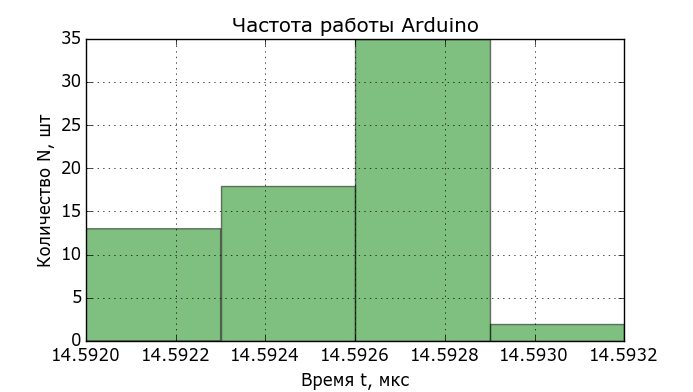
\includegraphics[width=.8\linewidth]{Figures/ardhist.png}
    \caption{Гистограмма измерений частоты Arduino}
    \label{fig:ardhist}
\end{figure}

Другими словами, дли включения и выключения одного выхода микроконтроллера \textbf{10000} раз нам понадобилось \textbf{145928} микросекунд, или \textbf{146} миллисекунд.

Одно включение и выключение выхода занимает $\frac{145928}{10000} = 14.5928$ микросекунд. Таким образом, \textbf{arduino} может выдавать сигнал с максимальной частотой

\begin{equation}
    \label{eq:freq1}
    \nu = \frac{n}{t} = \frac{10000}{145928 \cdot 10^{-6}} = 68526~\textrm{Гц} = 68.5~\textrm{кГц}
\end{equation}
